\chapter{Experiments}
\label{sec:chapterlabel4}

In the previous chapter, deep reinforcement learning agents were described to solve the recommendation task. Now, in order to test and evaluate their performance, a simulated environment for Recommender Systems is going be defined. Then, after defining the baseline models and the experimental settings, two sets of experiments are carried out: (i) a performance evaluation of the proposed deep learning models and a pure Collaborative Filtering baseline model; and (ii) an analysis of the convergence and speed-up between the deep reinforcement learning agent based on previous work in the area, and an DRL agent with the new policy approach. Final conclusions on the experimental results obtained will be presented in the next chapter.

\section{Reinforcement Learning Environment}

For the purpose to demonstrate how the deep reinforcement learning agent perform on the recommendation task, a simulated environment is modelled under the OpenAI Gym\footnote{\url{https://gym.openai.com/}} reinforcement learning toolkit. It that allow us to define Partially Observed MDP environments (POMDPs)  under an episodic setting where the agent's experience is broken down into a series of episodes\cite{brockman2016openai}. In general, OpenAI Gym manages two core concepts: (1) a free-to-code \textit{agent} that maximizes the convenience for users allowing them to implementation different styles of agent interface; and (2) a common \textit{environment} and action/observation interfaces that ease the implementation and testing of different reinforcement learning problems under the same framework. The final goal in OpenAI Gym is to maximize the expectation of total reward per episode, and to achieve a high level of performance in as few episodes as possible.

During each episode, the agent's initial state is randomly sampled from a distribution, and the interaction proceeds until the environment reaches a terminal state. After performing an action step, the environment interface returns the observation of current state, the reward achieved by the action performed, a done flag indicating if an episode ends and an information object containing useful information for debugging and learning. Finally, the framework also allow us to measure the performance of a RL algorithm under an environment along two axes: \textit{final performance} or average reward per episode, after learning is complete; and, \textit{sample complexity} or the amount of time it takes to learn. 

\subsection{Recommender System Environment}

The recommender system environment, characterized by a set of \textit{n} items to recommend to \textit{m} users, is defined (based on a previous definition in \cite{Dulac-Arnold2015}) as a sequence of MDPs $\langle \mathcal{A}, \mathcal{S}, r, \mathcal{P} \rangle$ composed by an action set $\mathcal{A}$ that correspond to set of items to recommend, a state space $\mathcal{S}$ holding the item the user is currently consuming, a reward $r$ defined as the rating value given by a user to an item if she accepts it, and a transition probability matrix $\mathcal{W}$ which defines the probability of that a user will accept item \textit{j} given that the last item she accepted was item \textit{i}. 

The transition probability matrix is generated using the ideas exposed by Yildirim et al. in \cite{yildirim2008random} to build a random walk recommender system using a Markov Chain mode,l where the probability of being in a state only depends on the previous step $Pr(X_{u, k+1} = i | X_{u, k})$. The algorithm presented in Appendix \ref{app:trans_prob_alg} details the underlying process to set up the environment.

\subsection {Simulation algorithm}

The implemented algorithm is presented in Appendix \ref{app:simulated_env} and describes the complete simulation process of the recommendation task. At each time-step, the agent presents an item \textit{i} to the user with action $\mathcal{A}_i$. The user then accepts the item according to the transition probability matrix $\mathcal{P}$ or selects a random item. To simulate the user patience in a session as in \cite{Dulac-Arnold2015}, an episode of learning ends with probability 0.1 if the user accepts the item, and with probability 0.2 if a random item is selected instead. Finally, after each episode the environment is reset by selecting a random item from a likely subset for an specific user provided by a single item-based collaborative filtering model based on the similarity between items.

\section{Data Set}

The 1M Movielens dataset \cite{harper2016movielens} from the GroupLens Reseach Lab\footnote{\url{http://grouplens.org/datasets/movielens/}} is used to train and test the implemented deep reinforcement agents. Table \ref{table:dataset} summarizes the statistical nature of the dataset. The ratings file was pre-processed in order to generate the user rating matrix, the transition probability matrix and to train and test the baseline CF-model using 5-fold cross validation to predict the missing ratings under the simulated environment.

\begin{table}[!htbp]
%\begin{center}
\centering
\begin{tabular}{ |l|r| }
  \hline
  \multicolumn{2}{|c|}{1M Movielens dataset} \\
  \hline
  Total ratings & 1,000,029 \\
  Users & 6,040 \\
  Movies & 3,883 \\
  Sparsity Level & 57.4\% \\
  Mean ratings/user & 165 \\
  Min. ratings/user & 20 \\
  Max. ratings/user & 2314 \\
  \hline
\end{tabular}
%\end{center}
\caption{Properties of the 1M Movielens dataset}
\label{table:dataset}
\end{table}

\section{Evaluation Scheme}

\section{Baselines and Experimental Settings}

To evaluate the strength and accuracy of deep reinforcement learning model, we compare the new model against a pure CF model and two variants of the baseline model described in section \ref{sec:baseline}, The description of each model is listed as follows:

\begin{itemize}
\item \textbf{FM-MCMC}: \textit{Factorization Machine with Monte Carlo Markov Chain inference}  uses FM based on the Bayeasian inference with a Gibbs sampling technique that generates the distribution of $\hat{y}$ by sampling the conditional posterior distribution for each model parameter. This model was chosen as the baseline model for comparison as it it outperforms other learning approaches like SGD and ALS, and also because it integrates the regularization parameter into the model, which avoids a time-consuming search for the optimal hyperparameters. The only hyperparameter that remains for MCMC is the initialization of the standard deviation$\sigma$ for the Gibbs sampler.
\item \textbf{DRL-kNN-CB}: \textit{DRL with Content-based similarity for continuous action spaces} model uses the DDPG algorithm with a bag-of-words feature vectors to represent actions and states. The k-nearest neighbors index is then created using a KDtree algorithm[***] to find the closest set of existing items from the action estimated by the actor function. Finally, the Wolpertinger policy will apply the action in $\mathcal{A}$ that yields to the maximum return.
\item \textbf{DRL-kNN-CF}: \textit{DRL with Item-based similarity} model uses a similar configuration as the model described above but it implements an item-to item version of the k-NN algorithm for CF using the item vectors from the user rating matrix to find the closest set of items from an action given by the actor function.
\item \textbf{DRL-FM}: \textit{DRL with Factorization Machines policy} model replaces the k-NN algorithm from the models previously described with the FM-BRP model to return the Top-k items that can be recommended from a given state. Then, the FM-policy will apply the action from the top-N recommendations that yields to the highest Q value in the long term.
\end{itemize}

For the content-based model, feature vectors for each item were created using a combination of word embeddings extracted using \textit{word2vec}\footnote{\url{https://radimrehurek.com/gensim/index.html}}, and genre categorization as a binary vector.

For the FM models, we use the \textit{fastFM}\footnote{\url{https://github.com/ibayer/fastFM}} library introduced by Bayer I. in \cite{bayer2015fastfm} that offers an efficient python implementationn of the FM learning algorithms including MCMC and BRP-OPT with SGDthe ratings file was transformed to the $SVM^{light}$ representation introduced in \cite{joachims1999making}. Figure \ref{fig:featurevector} shows an example of the feature vector representation. First, there are $|\mathcal{U}|$ binary indicators variables (blue) that represent the active user of a transaction. The next $|\mathcal{I}|$ binary indicator variables (red) hold the active item. Each feature vector also contains normalized indicator variables (yellow) for all other items the user has ever rated. Finally, the vector contains a variable (green) holding the time when the rating was registered, and another variable containing information of the last movie the user has rated before.

In the experiments, (hyperparameter configuration for each model)[***Missing]

\begin{figure}[h]
\centering
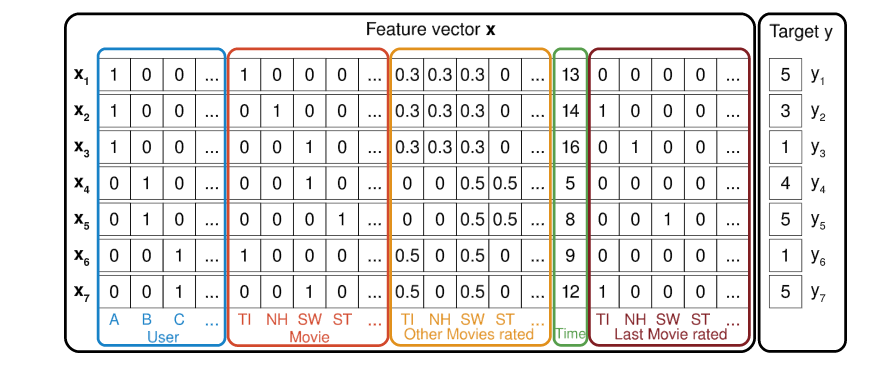
\includegraphics[scale=0.9]{images/featurevectors}
\caption[Feature vector representation in the $SVM^{light}$ format]{Feature vector representation for ratings under the FM models (Source: Factorization machines\cite{rendle2010factorization})}
\label{fig:featurevector}
\end{figure}

\section{Results}
